\section{Theory}
The measurement of the elementary charge, denoted by $e$,
is a fundamental milestone in physics that provides deep
insights into the quantized nature of electric charge. The
Millikan oil drop experiment, first conducted by Robert
A. Millikan in 1909, is one of the most famous experiments designed to measure this quantity with precision.
Prior to Millikan's work, the existence of a smallest unit
of charge was hypothesized but not conclusively proven.
Millikan's experiment provided the first direct and accurate measurement of $e$, supporting the atomic theory of
matter and the discrete nature of electric charge.

In the experiment, tiny oil droplets are introduced into
a chamber where they are subjected to gravitational and
electric forces. By adjusting the electric field, a droplet
can be suspended in equilibrium, allowing the charge
on the droplet to be determined. By observing multiple droplets, Millikan was able to show that the charges
on the droplets were all integer multiples of a fundamental unit of charge, which he identified as the elementary
charge. The significance of this experiment extends beyond the measurement of $e$; it also confirmed the quantization of charge, a key principle in modern physics. The
Millikan oil drop method remains a classic demonstration
of experimental ingenuity and precision in the study of
fundamental physical constants.

\subsection*{Experimental Process}

Consider a spherical oil droplet of radius $r$ and density
$\rho$ falling under the gravitational force. This droplet in
air is acted upon by a constant force and soon reaches
a terminal velocity given by Stoke's law, 

\begin{align}F_\nu = 6\pi \nu rv_f\end{align}

where $\nu$ is the coefficient of viscosity of air and $v_f$ is
the terminal velocity during the fall. The gravitational
and buoyancy forces acting on the droplet are balanced
by $F_\nu$ (Fig. \ref{1}).

\begin{figure}[H]
    \centering
    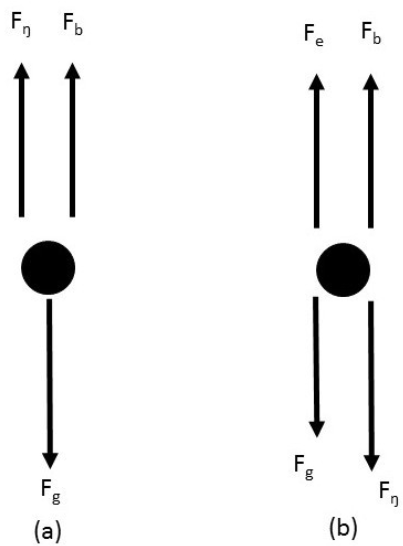
\includegraphics[width=.4\columnwidth]{images/1.png}
    \caption{Different forces acting on the oil droplet during (a) free fall and (b) rise of the droplet in the presence of an electric field.}
    \label{1}
\end{figure}

\begin{align} \label{eq1}
    \frac{4}{3}\pi r^3 \rho g - \frac{4}{3}\pi r^3 \rho_a g = 6\pi \nu rv_f
\end{align}

where $\rho_a$ is the density of air. The falling velocity $v_f$ is hence given by,

\begin{align} \label{eq2}
    v_f = \frac{2}{9} \frac{gr^2}{\nu} (\rho-\rho_a)
\end{align}

If the droplet carries a charge $ne$ and is moving upward
with terminal velocity $v_f$ under the influence of the applied electric field $V/d$ between the parallel plate electrodes separated by the distance $d$ and potential difference $V$, the force equation is

\begin{align} \label{eq3}
    \frac{4}{3}\pi r^3 (\rho-\rho_a) g + 6\pi \nu rv_f = \frac{Vne}{d}
\end{align}

Solving for $ne$, we subtract Eq. \ref{eq1} from Eq. \ref{eq3},

\begin{align} \label{eq4}
    ne = \frac{6\pi \nu rd}{V}(v_f-v_r)
\end{align}

Dividing Eq. \ref{eq4} by Eq. \ref{eq2},

\begin{align} \label{eq5}
    \boxed{ne = \frac{4\pi}{3}\frac{gd}{V}r^3(\rho-\rho_a)\left(1+\frac{v_r}{v_f}\right)}
\end{align}

The Stoke'’'s law used in obtaining Eqs. \ref{eq1} to \ref{eq5} assumes that the droplets are moving slowly, that there is no
slipping of the medium over the surface of the droplet,
that the medium is of quite large extent compared to
the size of the droplet and that the inhomogeneities in
the medium are of a size small compared to the size of
the droplets. In the present case all the assumptions
except the last one are reasonably valid. The radii of
the droplets are of the order of one micron and therefore not much greater than the mean free path of the air
molecules. The droplets will tend to fall more quickly in
the free space between the air molecules. The expression
for the falling velocity vf corrected for this effect on the
basis of kinetic theory is

\begin{align} \label{eq6}
    v_f = \frac{2}{9}\frac{gr^2}{\nu}(\rho-\rho_a)\left(1+\frac{C}{Pr}\right)
\end{align}
 
where $C = 6.17 \times 10^{-8}$ m of Hg-m is a correction factor and P (in m of Hg) is the atmospheric pressure. If we write,

\begin{align}
    \xi &= \frac{9\nu}{2g}\frac{v_f}{\rho-\rho_a}\\
    \zeta &= \frac{C}{2P}\\
    \text{Eq. 7 becomes, } &r^2 + 2\zeta r - \xi = 0
\end{align}

The radius of the droplet is given by the positive root of this equation

\begin{align}
    r = -\zeta + \sqrt{\zeta^2+\xi}
\end{align}

The charge ne may be obtained by first calculating $\xi$ and
$\zeta$ from Eqs. 8 and 9, then calculating the radius $r$ from Eq. 11 and finally $ne$ from Eq. 6. Equation 5 above is for the Dynamic method. In the Balancing
method, the droplet is kept stationary by adjusting the
potential. The upward velocity is thus equal to zero. The
final equation for $ne$ in the Balancing method is therefore

\begin{align}
    \boxed{ne = \frac{4\pi}{3}\frac{gd}{V_b}(\rho-\rho_a)r^3}
\end{align}

where, $V_b$ is the balancing potential Time for free-fall of
the droplets under gravity between the preset points is
measured to obtain the velocity for free- fall. For observing the effect of the electric field on the charge carried by
the droplets, there are two alternatives. In the Dynamic
method, the velocity for the vertical upward motion is
measured for a fixed potential difference.

% ==============================================================
\section{Experimental Setup}

\subsection*{Apparatus}

\begin{enumerate}
    \item A oil drop chamber mounted on top of the panel. It has
    \begin{itemize}
        \item A pair of horizontal parallel plate electrodes
        separated by about 5 mm thick ebonite ring
        with a hole for viewing the oil droplets.
        \item The upper plate has a small hole in its centre for the admission of the droplets which are
        produces by spraying oil with an atomizer.
        \item A device to illuminate the space between the
        plate electrodes.
    \end{itemize}
    \item Three levelling screws at the base of the panel to
    make the parallel plate electrodes perfectly horizontal (perpendicular to the gravitational field) and a
    water-level placed on top of the panel to check it.
    \item A microscope with CCD camera head to view and
    transmit image of oil droplets between the plate electrodes to the monitor.
    \item A power pack to supply continuously variable voltage in the range 0 - 800 V to the upper plate electrode when the electric field is to be created between the plates.
    The lower plate is permanentl grounded.
    \item A digital voltmeter to measure the potential applied
    to the upper plate.
    \item A ‘Time Meter’ or a stopwatch to display the time for which the oil droplet is allowed to move.
    A monitor with graduated screen. The horizontal lines on the monitor screen help in setting the distance through which the droplets move.
    \item An atomizer to spray droplets.
\end{enumerate}

\begin{figure}[H]
    \centering
    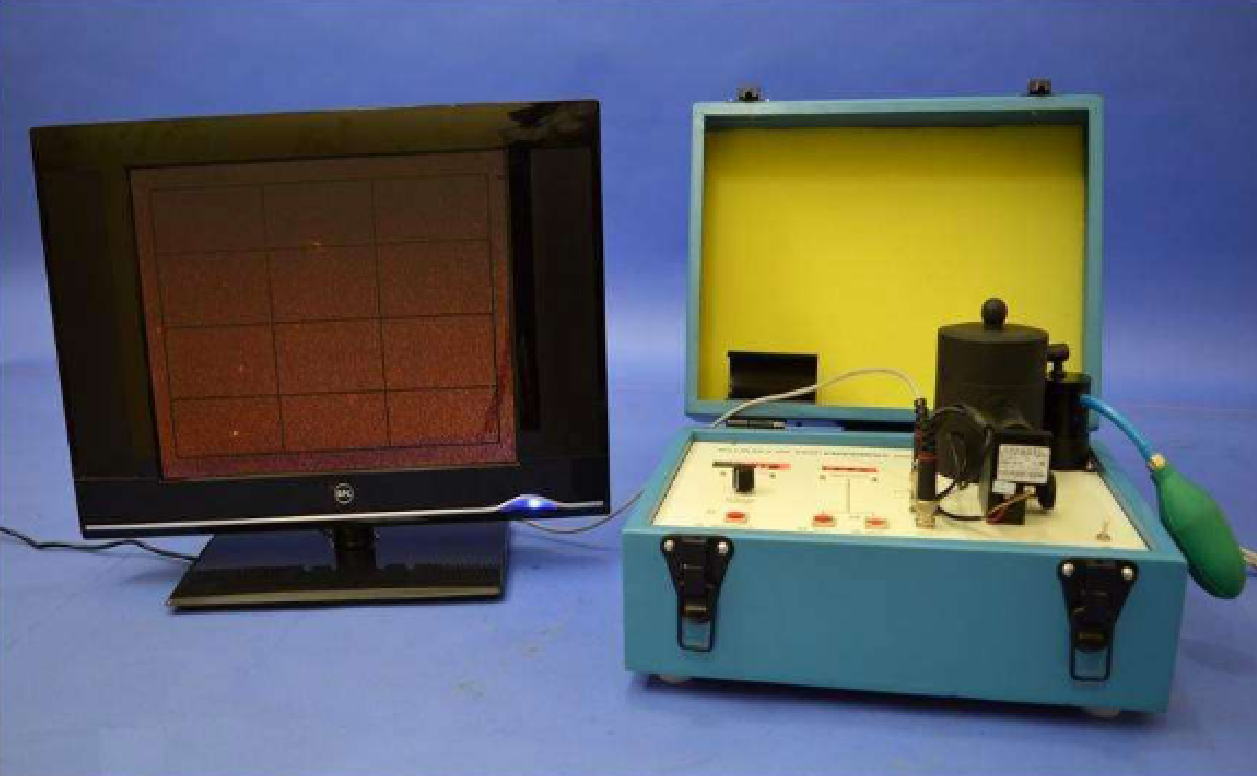
\includegraphics[width=.8\columnwidth]{images/2.png}
    \caption{The experiment set-up}
    \label{2}
\end{figure}